% Your name
\renewcommand{\YRname}{R. Oechslin}

% Your grade/post
\newcommand{\YRgrade}{M2}

% Submission date
\newcommand{\YRdate}{2018.Apr.27}

% Your research theme
\newcommand{\YRtheme}{Haptic Feedback Controller with Palm Pressurization}

% Work plan
\newcommand{\YRplan}{
	\hspace{-4truemm}
	\begin{tabularx}{170truemm}{|p{50truemm}||X|X|X|X|X|X|X|X|X|X|X|X|}
		\hline
		\multicolumn{13}{|c|}{\parbox[c][10truemm][c]{0truemm}{} \large Research theme: \bf \YRtheme} \\
		\hline
		\hline
		\multicolumn{13}{|c|}{\parbox[c][8truemm][c]{0truemm}{} \large \bf --- Research Plan ---} \\
		\hline
		Term \textbackslash Month & 2 & 3 & 4 & 5 & 6 & 7 & 8 & 9 & 10 & 11 & 12 & 1 \\
		\hline
		% For ``Work plan'', do not change above.
		\hline
		Literature review & & & & & & & & & & & & \\
		\shadecells{2-2}
		\hline
		Design PlayStation Controller  & & & & & & & & & & & & \\
		\shadecells{2-3}
		\hline
		Test PlayStation Controller & & & & & & & & & & & & \\
		\shadecells{4-5}
		\hline
		Design Pilot Controller & & & & & & & & & & & & \\
		\shadecells{2-4}
		\hline
		Test Pilot Controller & & & & & & & & & & & & \\
		\shadecells{4-6}
		\hline
		& & & & & & & & & & & & \\
		%\shadecells{2-10}
		\hline
		Program mbed device& & & & & & & & & & & & \\
		\shadecells{5-5}
		\hline
		Redo experiments & & & & & & & & & & & & \\
		\shadecells{5-6}
		\hline
		Make third controller? & & & & & & & & & & & & \\
		\shadecells{5-7}
		\hline
		Analyze data and compare& & & & & & & & & & & & \\
		\shadecells{7-8}
		\hline
		Write Thesis & & & & & & & & & & & & \\
		\shadecells{8-8}
		\hline
	\end{tabularx}
}

% Main contents of your work
\newcommand{\YRachievement}{
	\section{Introduction}
	A lot of research on haptic feedback in handheld devices has been conducted, not only with force feedback (\cite{Prattichizzo2012}, \cite{Schoonmaker2006}), but also with pressure stimulation (\cite{Asada2016}, \cite{Nakamura2016}). The major applications for such haptic feedback devices can be found in (minimally invasive) surgical teleoperated medical systems (\cite{Bedem2009}, \cite{Enayati2016}, \cite{Tavakoli2004}, \cite{Nisky2011}), mobile augmented reality (\cite{Bermejo2017}, \cite{Hasegawa2006}) and teleoperated robotic systems (for example in space) \cite{Christiansson2007}. However this research project focuses on implementing a feedback on a handheld controller for a non-specified group of grounded wheeled robots. The controller uses pressurization feedback as a substitution for force feedback to give an intuitive%TODO say what intuitive means, give maybe a dictionary definition
	 feeling about the intrinsic state of the robot. The tests of the controller shall be made on the commercially available crawler robot from topy \footnote{\url{http://www.topy.co.jp}} using two tracks as means of transportation.
	
	As an initial approach and to be consistent with the previous research in this area \cite{AsadaPre} the robots orientation (pitch and roll angles) have been taken as state of interest. As an alternative measure, the current in the two crawler motors can be fed back to the user, to have a rough idea of used energy and to make it detectable if the robot is being stuck or blocked somewhere.
	
	\subsection{Project Description and Status Quo in the Beginning of the Project}
	The handheld controller that has been designed at Yamamoto's lab in 2016 and 2017 uses voice coil motors (VCMs) for the feedback. The disadvantage of these motors is that a constant voltage has to be applied to maintain a constant force. This leads to an energy-inefficient system and produces a lot of extra heat. The testing environment for this controller consists in a Unity program that lets the user control a tank with crawlers in an artificial landscape. When one drives over the hills and smaller bumps, the user feels the magnitude of the tilt (orientation angles roll and pitch) as a pressure on the palms. \\
	The goal of this work is to replace the VCM by a set of series elastic actuators (SEAs). These SEAs should have a low backdriveability, such that the setup can maintain a feedback force without constantly applying a voltage. Different types of models using SEAs shall be prototyped and tested on a real robot (topy). Furthermore, different feedback laws shall be implemented and tested to find the most intuitive feedback for the state of the robot.
	
	\section{Design and Analysis}
	\subsection{Series Elastic Actuators}
	The principle of series elastic actuators is relatively simple. The concept is explained in \cite{Pratt1995} which also mentions a more accurate and stable force control and the possibility of energy storage. A thorough study of an SEA design and its analysis has been made in \cite{Junior2016}, stating that the most important parameter in the system is the spring constant. Therefore, springs with several different spring constants have been used for the analysis of this research project.\\
	In this study, two different SEA designs have been implemented and tested. The first design is based on a linear movement (constrained by a linear guideway), where the rotary motion of the motor is driving a lever, pushing the carriage back and forth. For more details, see figure \ref{fig:actuation_system_explained}. \\
	The second design is an approximated linear motion, due to a very large lever (rotational-L) actuated by a cam principle.
		
	\subsection{Design of the PlayStation Controller}
	The first design of the haptic feedback controller has been partially inspired by the existing design and partially by the commercial controllers of PlayStation. The controller can be seen in figure \ref{fig:centric_shaft_controller_smaller}.
	
	\begin{figure}[h!]
		\centering
		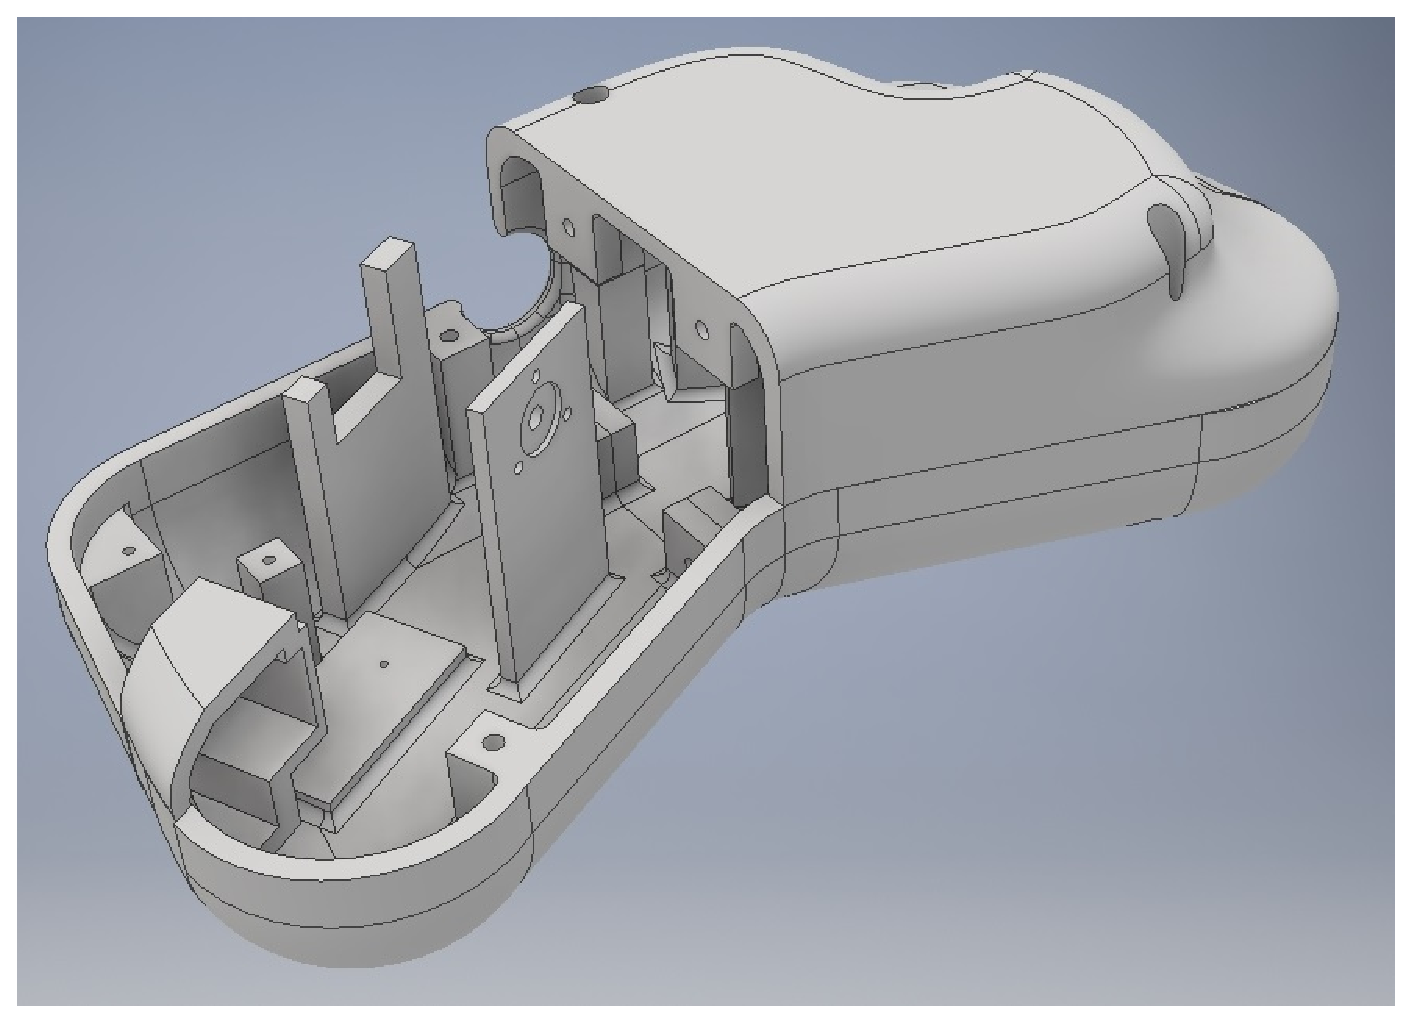
\includegraphics[width=0.6\linewidth]{Figs/centric_shaft_controller_smaller}
		\caption{3D model of the PlayStation controller.}
		\label{fig:centric_shaft_controller_smaller}
	\end{figure}
	
	This design of the controller aims at having a natural position for the hands, such that the user can hold the controller for a long time without having the hands in an awkward position. As it can be seen in the figure, the palm pads that transmit the feedback pressure to the palms are not directed perpendicularly towards the user, but rather outwards at a certain angle (refer to figure \ref{fig:centric_shaft_controller_smaller_top_view}). This can be seen as a drawback, since the user is expected to have the most intuitive feeling with a feedback opposing the driving direction (ie. perpendicular).
	\begin{figure}[h!]
		\centering
		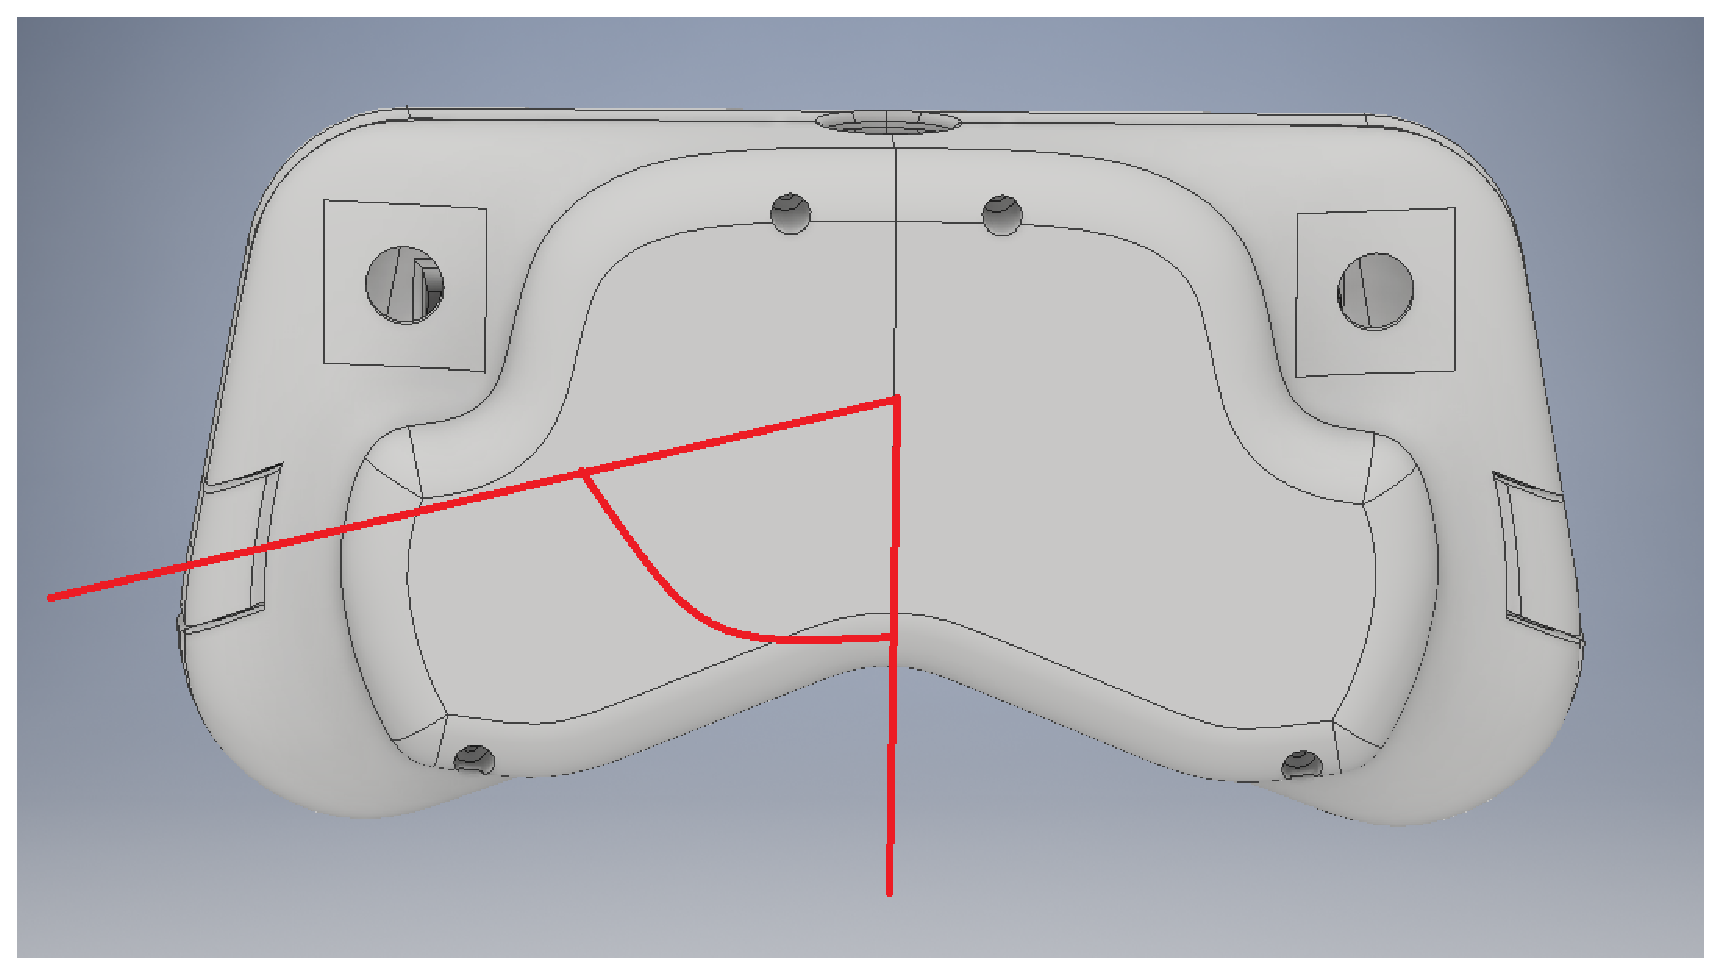
\includegraphics[width=0.7\linewidth]{Figs/centric_shaft_controller_smaller_top_view}
		\caption{3D model of the controller and the feedback direction indication.}
		\label{fig:centric_shaft_controller_smaller_top_view}
	\end{figure}
	
	
	The dimensions of the controller are 220mm in length, 110mm in width and 70mm in height. The controller is unusually thick due to the feedback actuation design. This actuation design can be seen in figure \ref{fig:actuation_system_explained}. The motor shaft is rotating a clamp link which is attached to a 3D-printed part, called connecting link. This 3D-printed part is attached to the carriage, an also 3D-printed part called L-plate, and is screwed to the linear guideway. The L-plate is connected via a set of springs (of variable spring constants) to the palm pad, thus making it an SEA. The linear guideway keeps the palm pad in a linear motion.
	\begin{figure}[h!]
		\centering
		\includegraphics[width=0.4\linewidth]{Figs/actuation_system_explained}
		\caption{Actuation system with legend.}
		\label{fig:actuation_system_explained}
	\end{figure}

	The legend refering to the actuation system in figure \ref{fig:actuation_system_explained} is as follows:
	\begin{itemize}
		\item (1) : Palm pad
		\item (2) : Photoreceptor
		\item (3) : L-plate
		\item (4) : Connecting link
		\item (5) : Clamp link
		\item (6) : Motors
		\item (7) : Linear guideway
		\item (8) : Springs
	\end{itemize}
	
	
	\subsubsection{Design of the Pilot Controller}
	The 3D model of the left-hand side pilot-based controller can be seen in figure \ref{fig:left_hand_joystick_cam}. To see the inside of the controller, the cover has been removed. To assemble it three sets of screws and nuts are necessary, making it easy to assemble and take apart. Also, this design is smaller in volume than the PlayStation controller. It is therefore more slender, cheaper and faster to manufacture.
	\begin{figure}[h!]
		\centering
		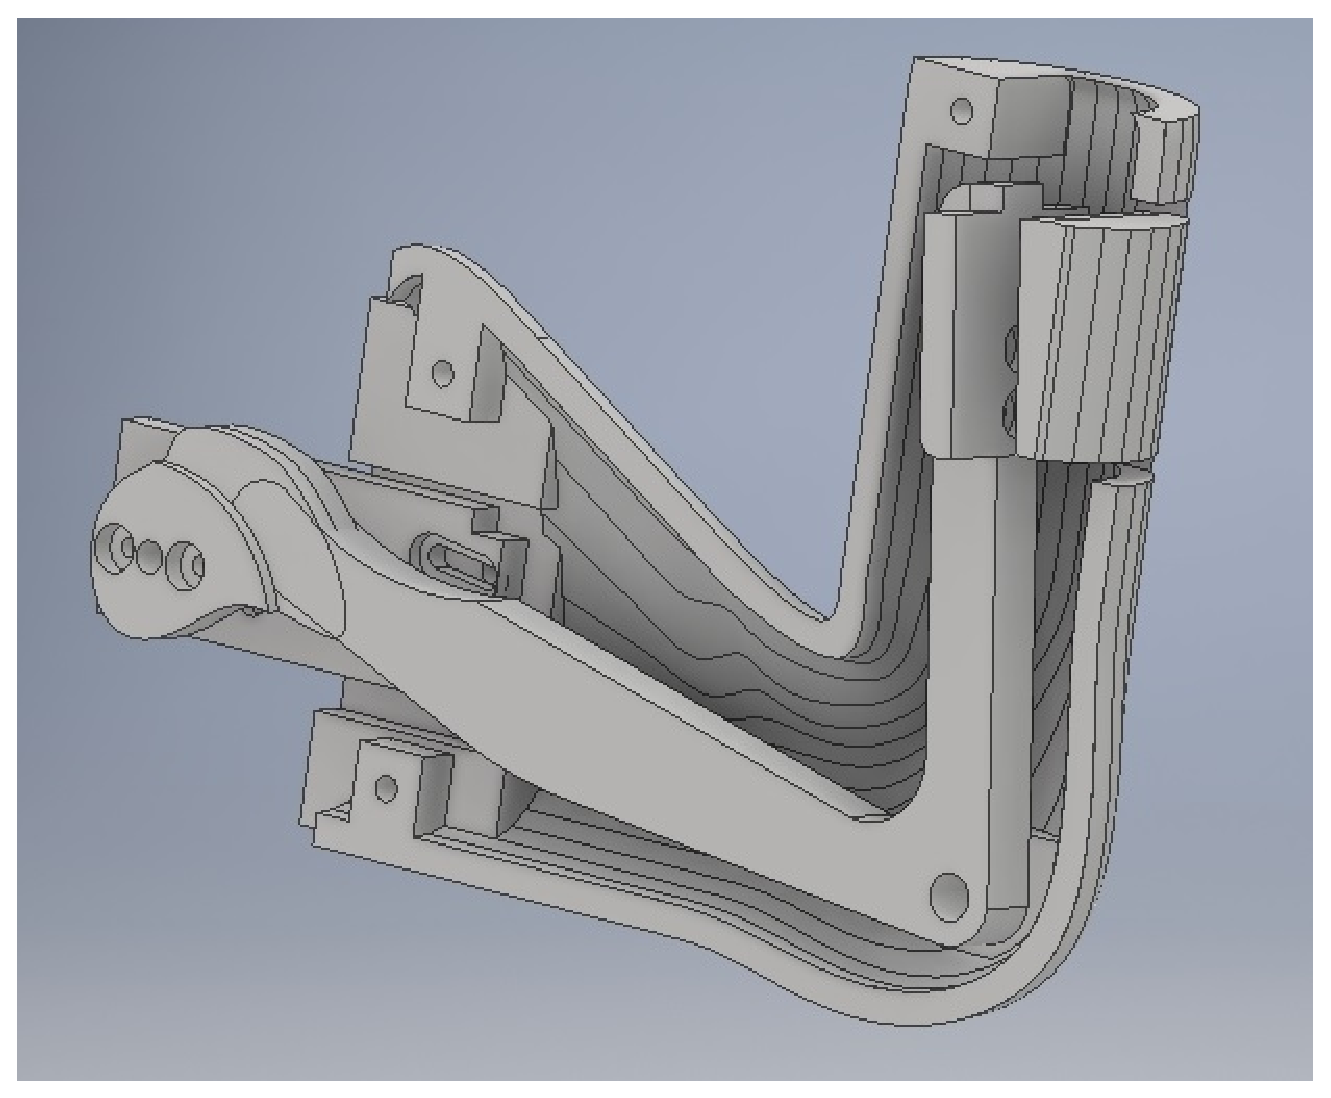
\includegraphics[width=0.4\linewidth]{Figs/left_hand_joystick_cam}
		\caption{3D model of the left-hand side controller with a removed cover.}
		\label{fig:left_hand_joystick_cam}
	\end{figure}

	In this design, the feedback motion is perpendicular towards the user and opposing the direction of motion. However, there is a slight angle at which the force is acting, due to the rotational design in the controller. But due to the large lever, this effect can be neglected. The actuation principle is based on a simple cam disk that directly pushes the rotational-L. For this design, the motors with a higher reduction gear ratio have been foreseen.
	
	
	\subsection{Test Environment and Programs}
	To test the controller, it was necessary to write a properly working environment. The topy robot is communicating via a wireless serial link. It has a prespecified communication message that consists in $70$ bytes for sending from the robot to the PC and $44$ bytes for message to receive. These messages include the bytes reserved for proper starting and ending as well as the checksum. \\
	It was thus necessary to write an application that reads out the position of the two joysticks (basic potentiometers principle) and construct a message including these joystick values as speed reference for the robot. Then the message has to be sent over the wireless serial link to the robot and the answer has to be received. The important sensor readings (inclination, current in the crawlers, passed time and battery level) have to be read out and a feedback according to the chosen feedback law has to be sent to the motors.\\
	For this purpose, the programming language processing \footnote{\url{https://processing.org/}} has been used to create a graphical user interface and to establish the serial connection. For low-level motor control purposes an Arduino Uno has been used. The parameters that can be set for testing purposes can be seen in table \ref{tab:programming_params}.
	
	\begin{figure}[h!]
		\centering
		\begin{tabular}{|l|c|l|}
			
			\hline
			Setting & Value & Units \\ \hline \hline
			Baud rate for robot serial link & $9600$ & [bps]\\ \hline
			Baud rate for Arduino serial link & $9600$ & [bps] \\ \hline
			Update rate of the processing GUI & $5$ & [Hz] \\ \hline
			Update rate of the Arduino motor controller (in theory) & $200$ & [Hz] \\ \hline
			Update rate of the Arduino motor controller (in practice) & $170$ & [Hz] \\ \hline %TODO this should be in measured not in set parameters
			Max voltage for motor & $20$ & [V] \\ \hline
			Feedback resolution & 5 out of 255 & [-] \\ \hline
			PWM frequency & $31372.55$ & [Hz]  \\ \hline
			Proportional motor gain & $1.5$  & [-] \\ \hline
			Integral motor gain & $0.0$  & [-]\\ \hline
			Derivative motor gain & $0.0$  & [-]\\ \hline
			Feedback filter  & $50$ & [\%] \\ \hline %TODO calculate cut off frequency
			Left photoreceptor MIN value & $500$ & [-] \\ \hline %TODO explain more in detail what these values mean
			Left photoreceptor MAX value & $770$ & [-] \\ \hline
			Right photoreceptor MIN value & $680$ & [-] \\ \hline
			Right photoreceptor MAX value & $770$ & [-] \\ \hline			
		\end{tabular}
		\caption{Software parameters.}
		\label{tab:programming_params}
	\end{figure}
	
	\subsection{GUI in Processing}
	The graphical user interface shows the current feedback method as well as the magnitude. It also indicates which driving direction (forward, backward or halt) is sent to the robot. Since there is no control of the battery charge in the robot, it sends battery information in its message to the PC. The processing program reads out the charge of the battery and warns the user if it is too low. It stops the program, if the battery state is critical. The feedback method can be changed by a mouse-click anywhere in the window. The GUI can be seen in figure \ref{fig:processing_gui}.
	 
	\begin{figure}[h!]
		\centering
		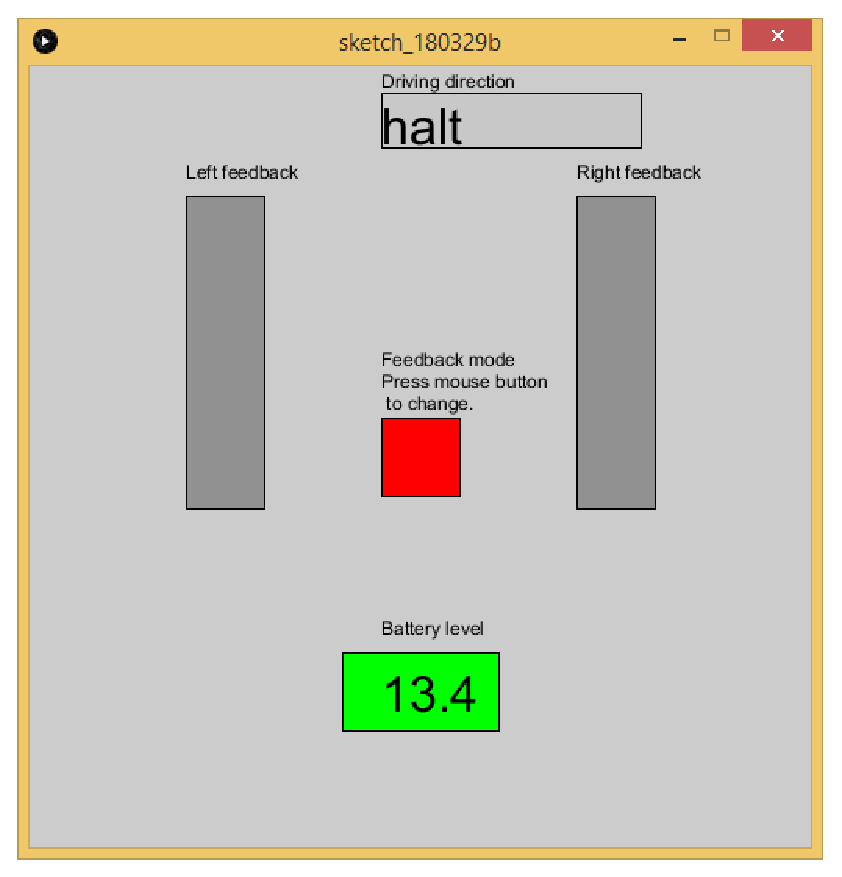
\includegraphics[width=0.4\linewidth]{Figs/processing_gui}
		\caption{Graphical user interface written in processing.}
		\label{fig:processing_gui}
	\end{figure}

	This application handles the messages sent to and from the robot.
	
	\subsection{Control Scheme}
	The control scheme is based on a simple proportional controller. The scheme can be seen in figure \ref{fig:control_scheme}. In the test setup the reference signal $dist_{ref}$ is given by the sinusoidal function generator. In the operational mode, this corresponds to the target output force, also called the haptic feedback force that should be felt by the user. Ideally, this shall be a function of orientation (roll and pitch) as well as the current in the two crawlers.
	\begin{figure}[h!]
		\centering
		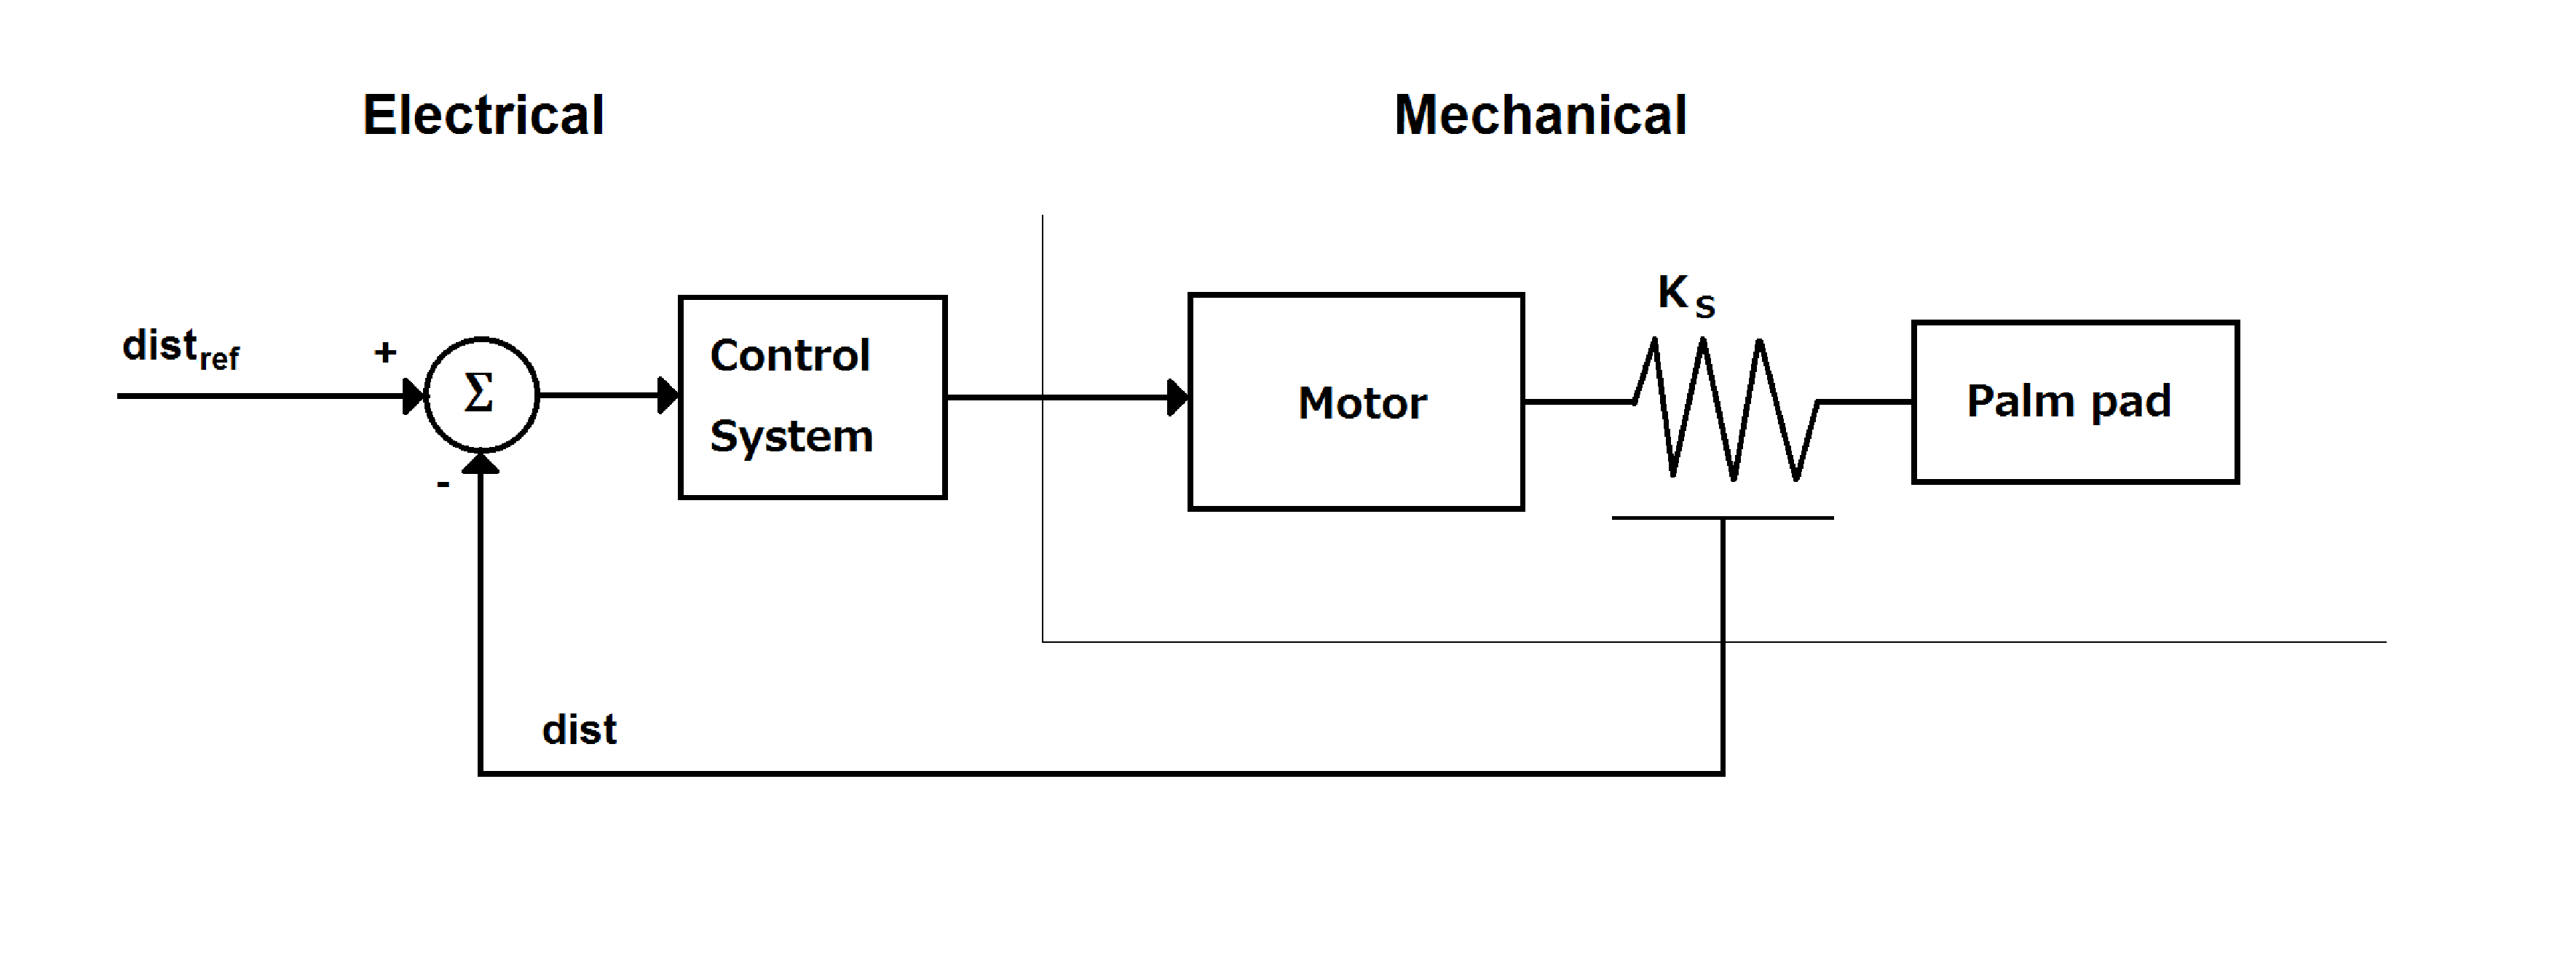
\includegraphics[width=0.7\linewidth]{Figs/control_scheme}
		\caption{Control scheme for the haptic feedback system.}
		\label{fig:control_scheme}
	\end{figure}
	
	\subsection{Electrical low-pass Filter}
	Before the PWM signal from the Arduino is sent to the amplifier, where it is amplified to control the motors, it has been filtered with a simple RC low-pass filter. The resistor has a value of $3.9$ k$\Omega$ and the capacitor of $0.1$ $\mu$F. This smooths out the PWM signal and has been implemented in order to avoid that the amplifier tries to follow the Arduino signal with unnecessary precision, eventually causing too much heat.
	
	
	\subsection{Photoreceptor Circuit}
	The photoreceptor that has been used is the TPR-105 from GENIXTEK CORP. Its sensing characteristics can be seen in figure \ref{fig:photoreceptor_curve}. The electrical circuit can be seen in figure \ref{fig:tpr105_circuit}. The component values are $R_1 = 330 \Omega$, $R_2 = 62$k$\Omega$ and $V_{CC} = 5$V. This receptor returns a $10$-bit value.
	
	\begin{figure}[h!]
		\centering
		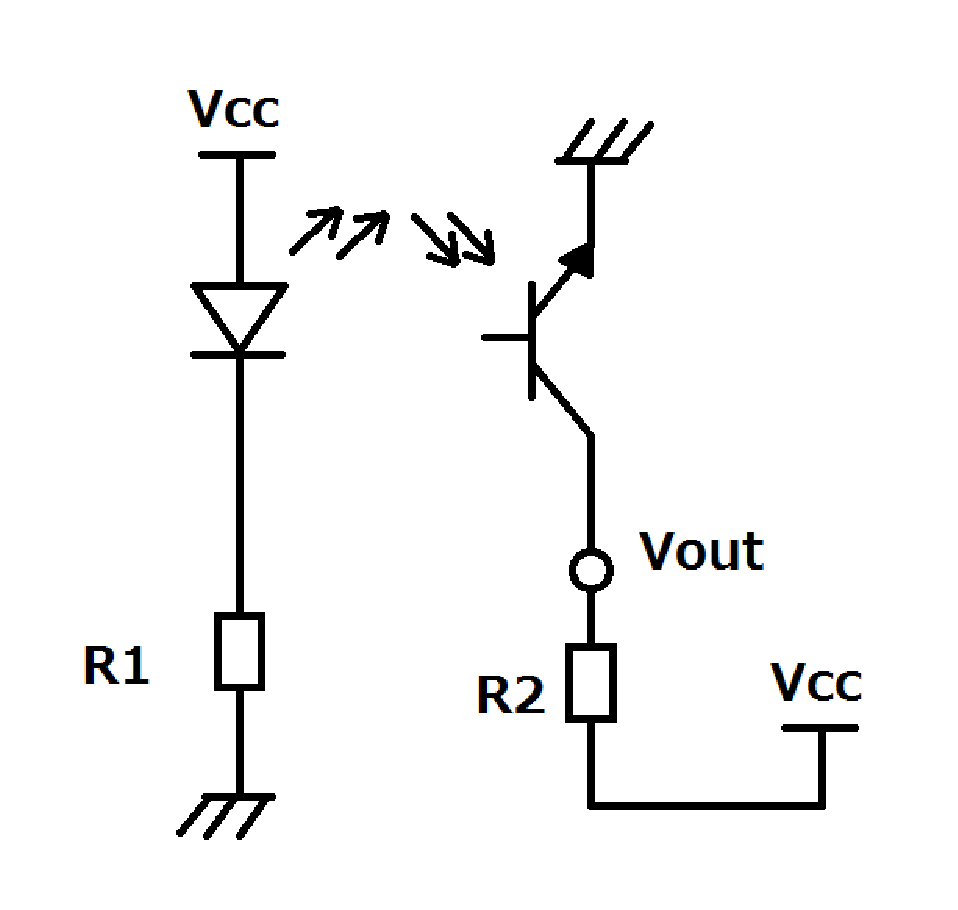
\includegraphics[width=0.2\linewidth]{Figs/tpr105_circuit}
		\caption{Implementation circuit of the photoreceptor.}
		\label{fig:tpr105_circuit}
	\end{figure}
	\begin{figure}[h!]
		\centering
		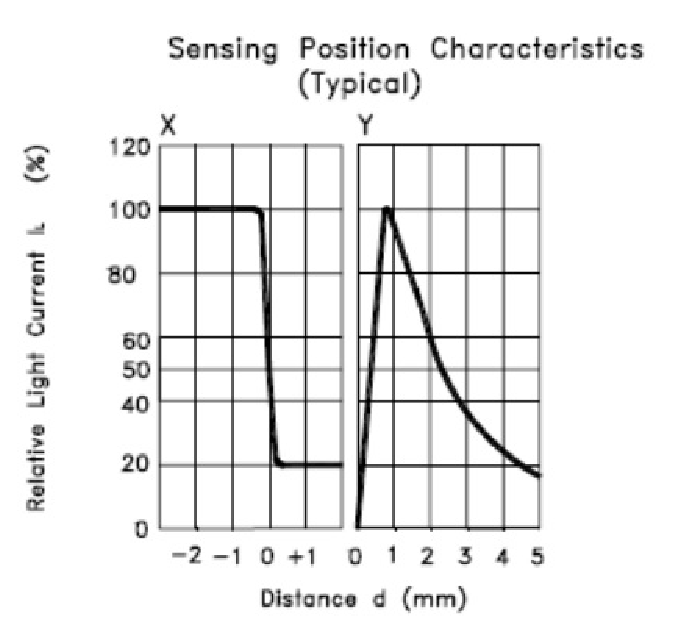
\includegraphics[width=0.3\linewidth]{Figs/photoreceptor_curve}
		\caption{Sensing characterstics of the photoreceptor TPR-105. Taken from its datasheet.}
		\label{fig:photoreceptor_curve}
	\end{figure}

	The sensing characteristics shows a nonlinear function in the range between $1$mm and $5$mm. However, as a first step, this has been interpolated linearly. To put it more precisely, the target output force has been mapped linearly to the measured distance. The operational distance lies between $4.5$mm to $5.5$mm.
	
	\section{Testing of the PlayStation Controller}
	For the two sides of the controller two different spring constants have been used. On the left-hand side, there is a set of three springs with a constant of $0.98$N/mm each. The motor has a reduction gear ratio of $33:1$. On the right-hand side the springs have a constant of $9.8 $N/mm and the motor has a reduction of $112:1$. The parameters are resumed in table \ref{tab:playstation_charac}.
	
	\begin{figure}[h!]
		\centering
		\begin{tabular}{|l|c|c|l|}
			\hline
			& Left side & Right side & Units\\ \hline \hline
			Clamp link length & 20 &  20 & [mm]  \\ \hline
			Motor reduction & $33:1$ & $112:1$ &  [-] \\ \hline
			Output torque (continous) & $30$ & $93$ & [mNm]  \\ \hline
			Output torque (intermittent) & $100$ & $180$ & [mNm] \\ \hline
			Number of springs used & $3$ & $3$ & [-] \\ \hline
			Spring constant & $0.9$ & $9.8$ & [N/mm] \\ \hline
			Equivalent spring constant & $2.7$ & $29.4$ & [N/mm] \\ \hline
		\end{tabular}
		\caption{Motor setup characteristics}
		\label{tab:playstation_charac}
	\end{figure}

	In order to conduct the frequency response analysis, the SG-4115 Function Generator has been used. The output signal was a sine wave with a peak-to-peak value of $2$V and an offset of $1.4$V. These settings have been made in order to stay within the detectable range of the Arduino $[0..5]$V. The frequency has been varied between $0.1$Hz and $35$Hz with $20$ logarithimcally spaced steps.
	
	Since the palm pads are blocked by the users hand in operational mode, they may not be considered blocked by an infinitely stiff wall. Therefore two different test setups have been created, where the palm pad has first been blocked by a screw driver in both directions, to have close to infinite stiffness, and a second setup, where the palm pads have been blocked by the users hands.
	
	\subsection{Results for Fixed Palm Pad Experiment (Pseudo Infinite Stiffness)}
	The input signal has been received as a feedback value (ie. $dist_{ref}$) and the P-controller stated in table \ref{tab:programming_params} controlled the output force by linearly mapping it to the photoreceptor distance. The measured distance has been logged and plotted. As it was expected, it is between the two extreme values stated in table \ref{tab:programming_params} (MIN and MAX). The response for the two extreme frequencies can be seen in figure \ref{fig:resp_left_hand_rigid_experim1}.
	\begin{figure}[h!]
		\centering
		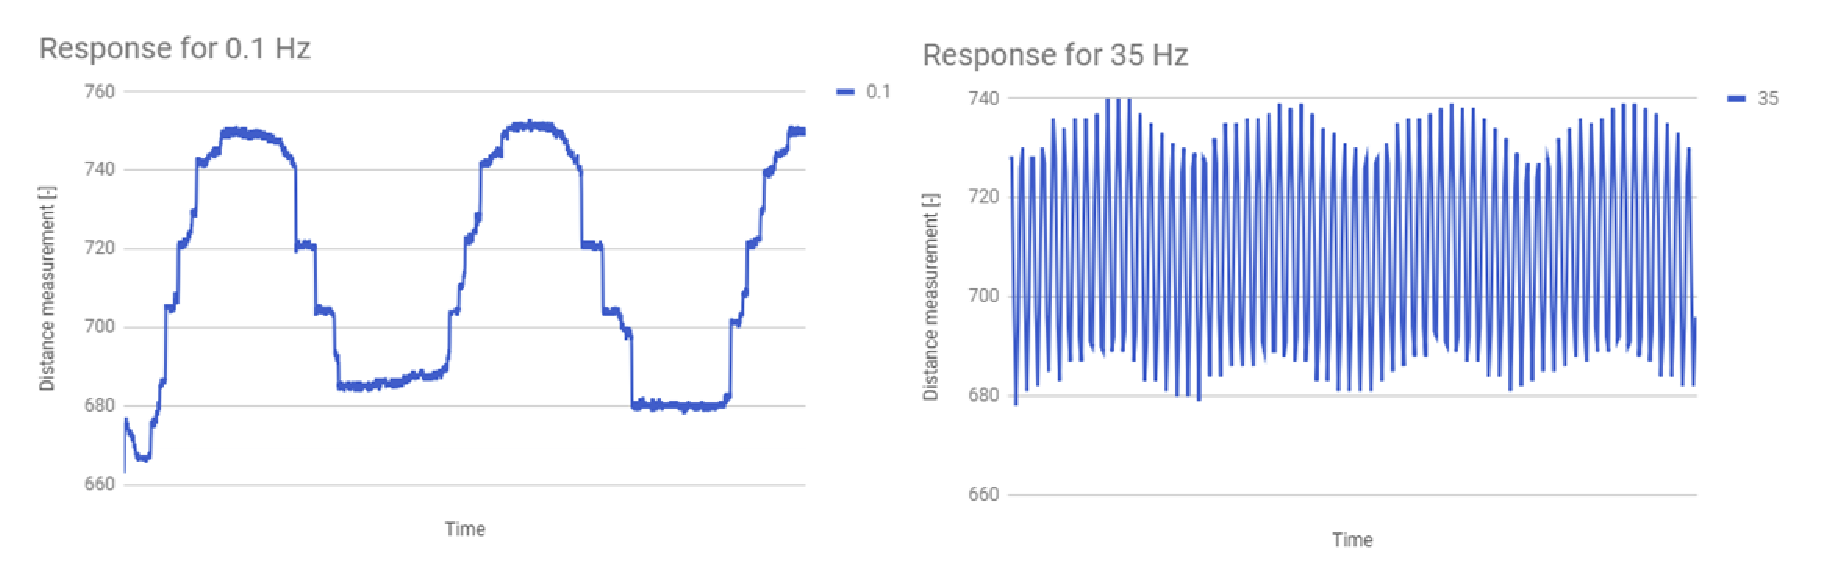
\includegraphics[width=0.7\linewidth]{Figs/resp_left_hand_rigid_experim1}
		\caption{}
		\label{fig:resp_left_hand_rigid_experim1}
	\end{figure}
	
	In order to find the frequency response, one is interested in the amplitude correlation between the input signal and the output signal, as given in the following equation:%TODO write how the FRF can be found, find a paper and reference it
	\begin{equation}
		H = \frac{F^*(j\omega)}{F(j\omega)}
	\end{equation}
	Where $F^*(j\omega)$ is the transfer function of the output signal and $F(j\omega)$ of the input signal.\\
	To calculate the amplitude of the output function (the measured value by the photoreceptor, corresponding to the distance between sensor and palm pad) one should ideally have a distinguishable value which is given by the maximal and minimal value of the sinusoidal output function. However, due to noise in the system, a sometimes occurring drift, interpolation aliasing and other effects such as the plateau characteristics shown in figure \ref{fig:resp_left_hand_rigid_experim1} and discussed in a later section, these minimum and maximum values are not clearly defined. Therefore, two different approaches have been chosen for the pseudo infinitely blocked palm pad experiment.
	
	First, the two quartile values ($Q_1$ and $Q_3$) have been calculated based on all the data, including outliers and noise. This is a relatively time-efficient method and is supposed to be less accurate since it sometimes includes errors such as the initial downward spike shown in the figure \ref{fig:resp_left_hand_rigid_experim1} for $0.1$Hz. The difference between these two quartile values has then been divided by the difference of the quartiles of the input signal ($Q_{3(sine)} - Q_{1(sine)}$). The results are indicated by the blue lines in figure \ref{fig:freq_resp_both_hands_rigid_experim1}.
	
	
	\begin{figure}[h!]
		\centering
		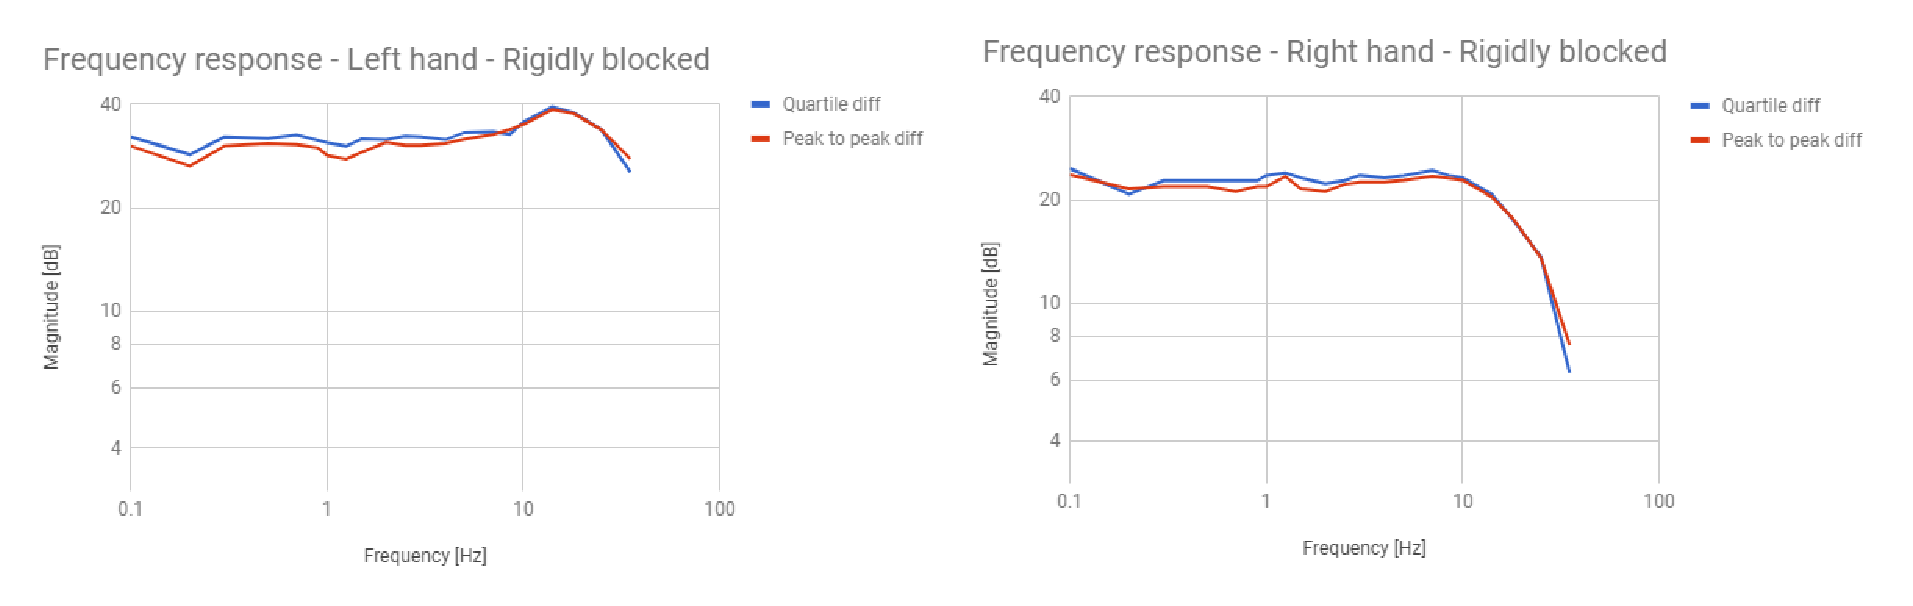
\includegraphics[width=1\linewidth]{Figs/freq_resp_both_hands_rigid_experim1}
		\caption{Frequency response analysis for both hands with a pseudo infinitely blocked palm pad.}
		\label{fig:freq_resp_both_hands_rigid_experim1}
	\end{figure}

	As an alternative output function, the amplitude has been measured manually, taking an average over several minima and maxima. This method is much more time consuming, but allows for filtering the noisy parts of the measurement, since it requires a visual representation of the measured data. These values are indicated on the same figure by the orange lines.
	
	\subsection{Results for Hand-Blocked Palm Pads Experiment}
	In the second experimental setup, the palm pads have been blocked by the hands of the user, to simulate an environment closer to the operational mode. This time, only the quartile method has been used to calculate the amplitude of the output signal. The results can be seen in figure \ref{fig:freq_resp_both_hands_soft_experim1}.
	\begin{figure}
		\centering
		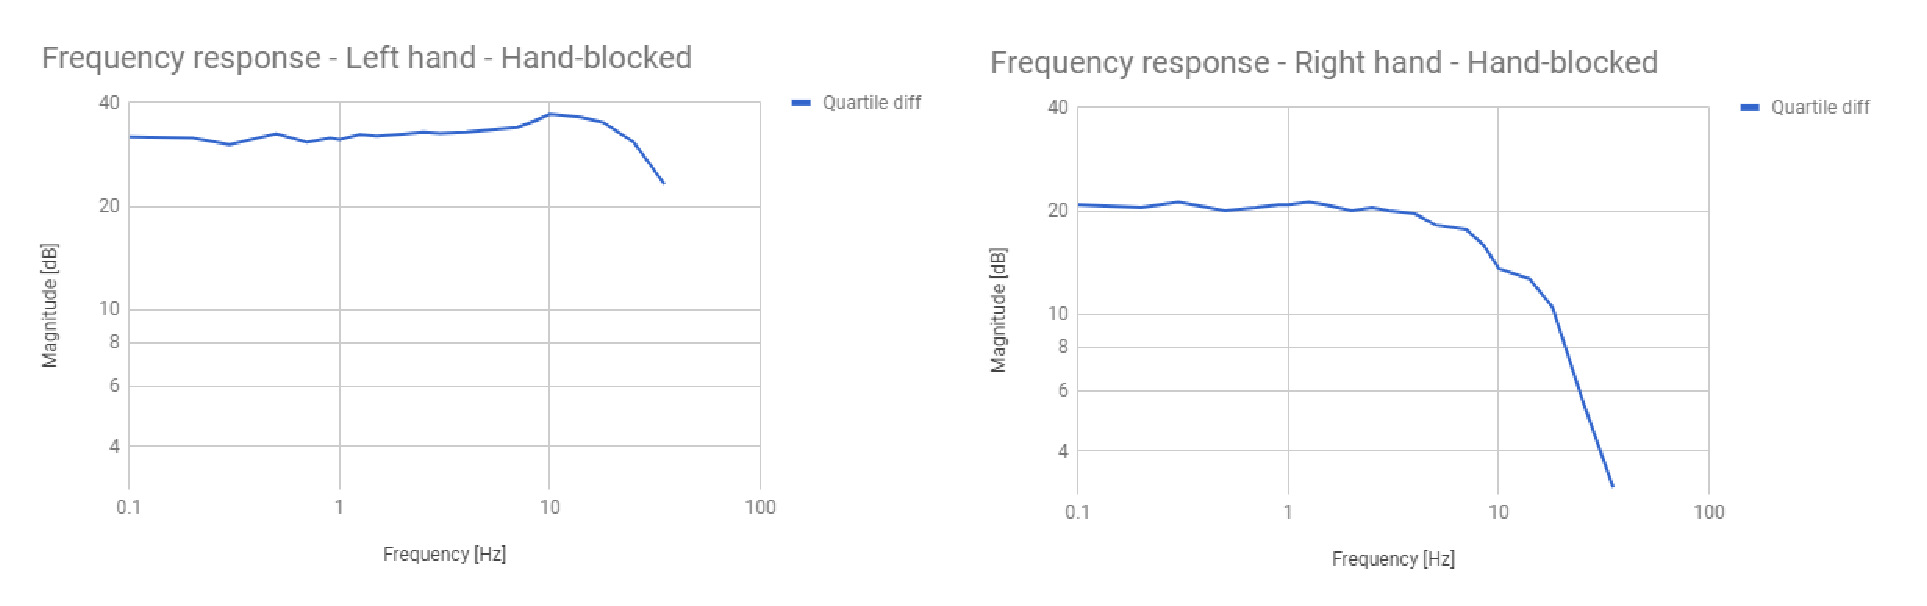
\includegraphics[width=1\linewidth]{Figs/freq_resp_both_hands_soft_experim1}
		\caption{Frequency response analysis for both hands with a hand-blocked palm pad.}
		\label{fig:freq_resp_both_hands_soft_experim1}
	\end{figure}
	
	The order of the system can be identified when looking at the slope of the Bode plot after its resonance top\footnote{Acutally, one should also consider the phase plot, but due to the reasons mentioned later in this research, this step has been skipped.}. This has been calculated for the six different curves and the following slopes have been found:
	
	\begin{tabular}{|c|c|c|}
		\hline 
		Rigid & left hand, blue line & $-54$ dB per dec \\ 
		\hline 
		& left hand, orange line & $-65$ dB per dec \\ 
		\hline 
		& right hand, blue line & $-54.8$ dB per dec \\ 
		\hline 
		& right hand, orange line & $-60.4$ dB per dec \\ 
		\hline 
		Soft & left hand & $-62.4$ dB per dec  \\ 
		\hline 
		& right hand & $-41.1$ dB per dec \\ 
		\hline 
	\end{tabular} 
	
	\section{Discussion}
	\subsection{Control Scheme and GUI}
	The control scheme is a simple proportional controller. It has been tested and decided to work well enough. If time permits, an integration and fine-tuning of an integral and derivative term can be done. \\
	There is not much to say about the GUI, however the handling of messages is not always done successfully. From time to time the processing program receives a message from the robot which is not complete. This results in accessing a cell of an array that is out of boundaries and the program crashes. To ensure the stability of the program, this case needs to be handled.
	
	\subsection{Design and Fabrication of the PlayStation Controller}
	The design of the controller is rather bulky and the actuation system might be too complex for what it is supposed to do. Due to its size, the upper and lower parts do not fit in the 3D printer and had to be cut in half and assembled by screws. This adds an extra step in manufacturing and assembly, making it more time-consuming. However the overall assembly is quite easy and tolerances have been chosen such that the whole system works. The feedback direction is not chosen optimally, if one aims at having a feedback opposing the driving direction (as seen from the robot).
	
	\subsection{Design and Fabrication of the Pilot Controller}
	This controller has almost been fully assembled, however not tested yet. It is much more simple to manufacture, as well as assemble. This design focused on having a feedback opposing the direction of motion.
	
	
	\subsection{Frequency Response Function}
	Figure \ref{fig:resp_left_hand_rigid_experim1} mainly shows two things. Firstly, there seems to be a certain step size, which is considerably more than expected. This results in only few values to attain for the photoeceptor, which can easily be seen in the response for $0.1$Hz. The second thing is, that at higher frequencies the Arduino has a too low update frequency and cannot follow the imposed sine signal, resulting in some aliasing effects. This shows that the Arduino is not capable of following frequencies higher than $35$Hz, but it also shows that the Arduino is not the right choice as a control device. The data analysis is therefore only to take with a grain of salt, since the important region after the resonance top had to be cut off. Future experiments shall be conducted using an mbed device, capable of operating at a control loop frequency of at least $1$kHz.
	
	As it can be seen in figure \ref{fig:freq_resp_both_hands_rigid_experim1} the two different methods of measuring the amplitude of the output signal share the same allures to a certain extent. This legitimizes to use the much more time-efficient approach of calculating the amplitude using the two quartile values. This argument has already been used for the data analysis in the experiment where the palm pads have been blocked by the users hand.
	
	The two figures \ref{fig:resp_left_hand_rigid_experim1} and \ref{fig:freq_resp_both_hands_rigid_experim1} show similar characteristics. Based on this, it seems appropriate to treat the two cases of pseudo infinite stiffness and hand-blocked palm pads as the same environment and for ease of analysis, only one of the two cases shall be treated.
	
	
	
	\section{Conclusion}
	The data that has been gathered with the Arduino as control device is only significant to a certain extent. The conclusions of using a screwdriver to block the palm pads for the experiments instead of the hand is still valid. However, the investigated frequency regions are too low to draw a meaningful conclusion and thus needs to be studied in more detail with a different control device (ie. an mbed). In addition to that, the phase diagrams have to be taken into account to confidently determine the order of the system.\\
	Furthermore, the most sensitive range of the photoreceptor is between $1$mm and $2$mm. The current implementation however is at a distance of roughly $5$mm making it much less linear and also less sensitive. This distance shall be reduced to increase linearity and sensitivity.
	
	
	\section{Outlook}
	First, the measured distance of the photoreceptor shall be changed to be in the range of $1.5$mm to $2.5$mm to have maximum linearity and sensitivity.\\
	The next step is to program the mbed to achieve the same control structure as with the Arduino, only with a higher control frequency. This should make it possible to study the system for higher frequencies. The control frequency shall be of $1$kHz, aiming for a maximum frequency of $100$Hz (Nyquist frequency is $f_s = 500$Hz and the practically achievable frequency is roughly one $5$th of this value).\\
	The experiments shall be conducted and analyzed again, this time also taking into account the phase plot in the Bode diagram. \\
	Additionally, the second controller shall be fully assembled and tested in the same manner.\\
	In parallel, the datasheet of the PMA servo motor driver shall be translated into English and the device integrated in the setup.

	
	%�����܂�
}


